\documentclass[compress,professionalfont]{beamer}
\mode<presentation>
\setbeamertemplate{navigation symbols}{}
\usetheme{Madrid}

% pdf is displayed in full screen mode automatically
\hypersetup{pdfpagemode=FullScreen}

\usepackage[utf8]{inputenc}
\usepackage[T2A]{fontenc}
\usepackage[russian]{babel}

\usepackage{graphics, graphicx}
\usepackage{amsmath}
\usepackage{amssymb}
\usepackage{amsfonts}
\usepackage{tikz,pgfplots}
\usepackage{pgfplots, epstopdf}
\usepackage{subfigure}
\usepackage{cmap}

\definecolor{darkred}{RGB}{16,78,139}
\newcommand{\myStandartColoredItem}[1]{{\color{darkred}\bf{{#1}}}}

\title[]{ПРИМЕНЕНИЕ МЕТОДОВ МАШИННОГО ОБУЧЕНИЯ ДЛЯ РЕШЕНИЯ ЗАДАЧИ ФИЛЬТРАЦИИ НЕЖЕЛАТЕЛЬНЫХ ДАННЫХ}
%\author[]{W. Hilberg\inst{1}, V.F. Kravchenko\inst{2,3}, Ya.Yu. Konovalov\inst{3}, O.V. Kravchenko\inst{2,3}}
%\institute[IRE]{TU Darmshtadt\inst{1}, IRE RAS named after V.A.~Kotelnikov\inst{2},\\ BMSTU named after N.E.~Bauman\inst{3}}
%\date{\today}
\author[Hilberg, Kravchenko, Konovalov]{Wolfgang~Hilberg\inst{1}, V.F.~Kravchenko\inst{2,3}, O.V.~Kravchenko\inst{2,3} \& Y.Y.~Konovalov\inst{3}}
\institute[]{Technische Universitat Darmstadt\inst{1}\\Kotel'nikov Institute of Radio Engineering and
Electronics of RAS\inst{2}\\ Bauman Moscow State Technical University\inst{3}}

\graphicspath{{images/}}

%%%%%%%%%%%%%%%%%%%%%%%%%%%%%%%%%%%%%%
\begin{document}
\begin{frame}[plain]
\titlepage
\end{frame}

%%%%%%%%%%%%%%%%%%%%%%%%%%%%%%%%%%%%%%
\begin{frame}
\frametitle{Актуальность проблемы}

\begin{center}

\includegraphics[width=0.45\textwidth]{actual1.jpg}
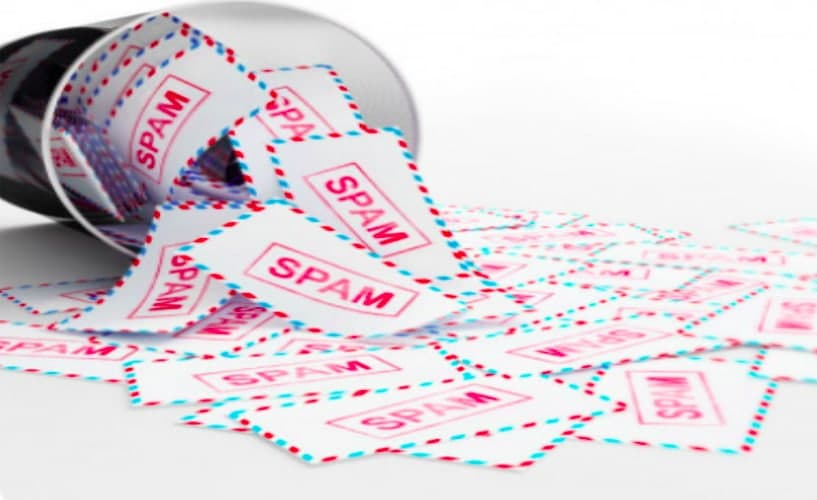
\includegraphics[width=0.45\textwidth]{actual2.jpg}
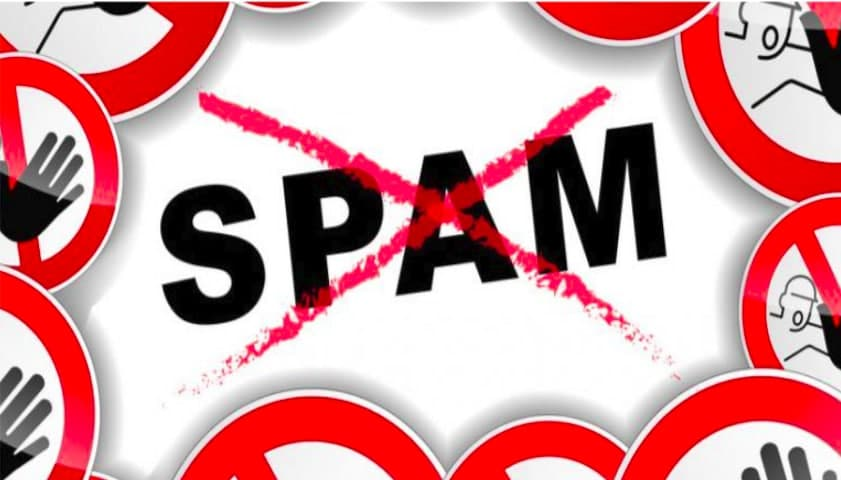
\includegraphics[width=0.45\textwidth]{actual3.jpg}

\includegraphics[width=0.45\textwidth]{actual4.jpg}
\end{center}
\end{frame}

%%%%%%%%%%%%%%%%%%%%%%%%%%%%%%%%%%%%%%
\begin{frame}
\frametitle{Постановка задачи}

В рамках работы требуется реализовать спам--фильтр для следующих продуктов Mail.Ru Group: почта, юла, мой мир, ответы, icq, пульс, агент. Ключевыми требованиями на фильтр являются:
\begin{itemize}
\item Высокая точность --- должно верно классифицироваться не менее 99\% писем.
\item Высокая отказоустойчивость --- сервис, осуществляющий запуск спам--фильтра, должен отвечать не менее чем на 99.99\% запросов.
\item Высокая производительность --- полный цикл проверки письма не должен быть дольше 3--х секунд.
\end{itemize}

Формально постановку задачи можно разбить на 4 этапа:
\begin{enumerate}
\item Предобработка письма.
\item Построение отображения текстовой информации в векторное пространство (векторизация).
\item Классификация объектов.
\item Постоение микросервисной архитектуры для запуска спам--фильтра на реальных пользователях.
\end{enumerate}

\end{frame}

%%%%%%%%%%%%%%%%%%%%%%%%%%%%%%%%%%%%%%
\begin{frame}
\frametitle{Предобработка}

\begin{center}
Предобработка
\end{center}

\end{frame}

%%%%%%%%%%%%%%%%%%%%%%%%%%%%%%%%%%%%%%
\begin{frame}
\frametitle{Предобработка}

Письмо в веб--интерфейсе
\begin{center}
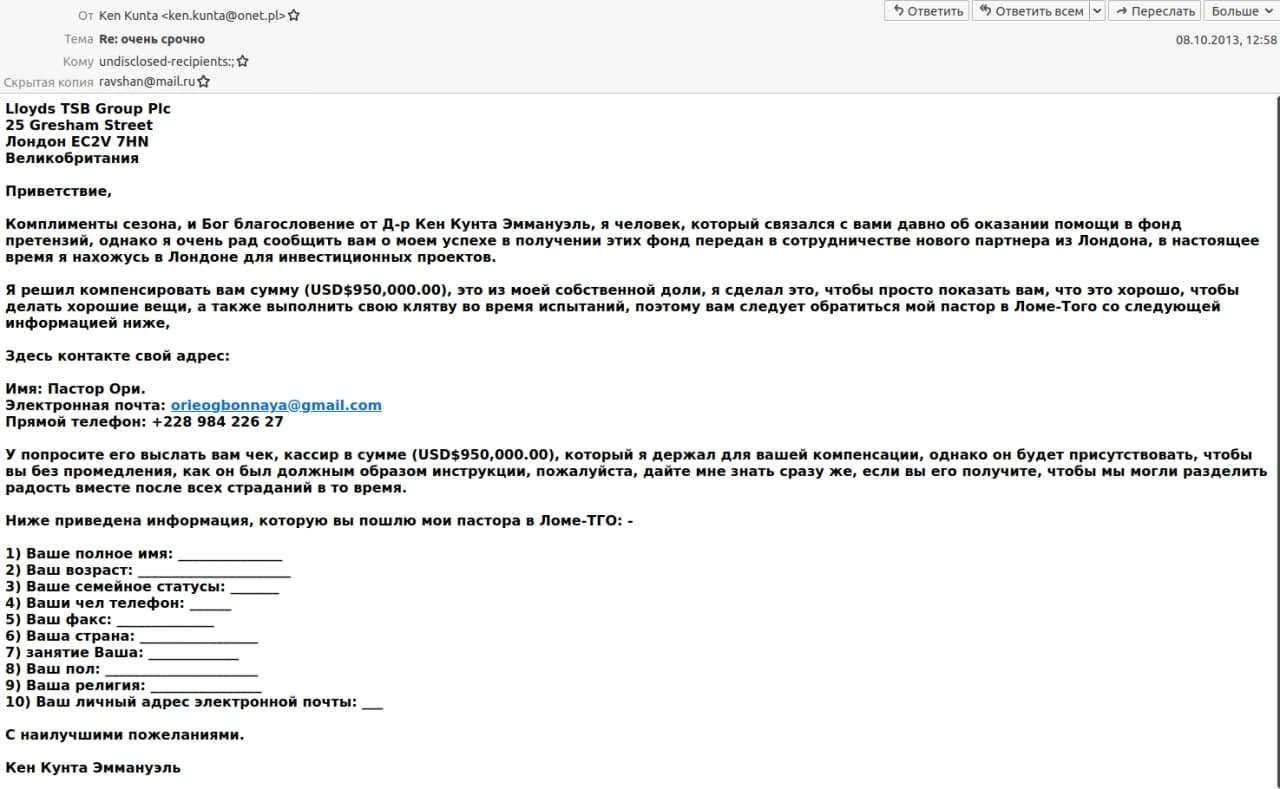
\includegraphics[width=.9\textwidth]{eml.jpg}
\end{center}

\end{frame}

%%%%%%%%%%%%%%%%%%%%%%%%%%%%%%%%%%%%%%
\begin{frame}
\frametitle{Предобработка}

Сырое письмо
\begin{center}
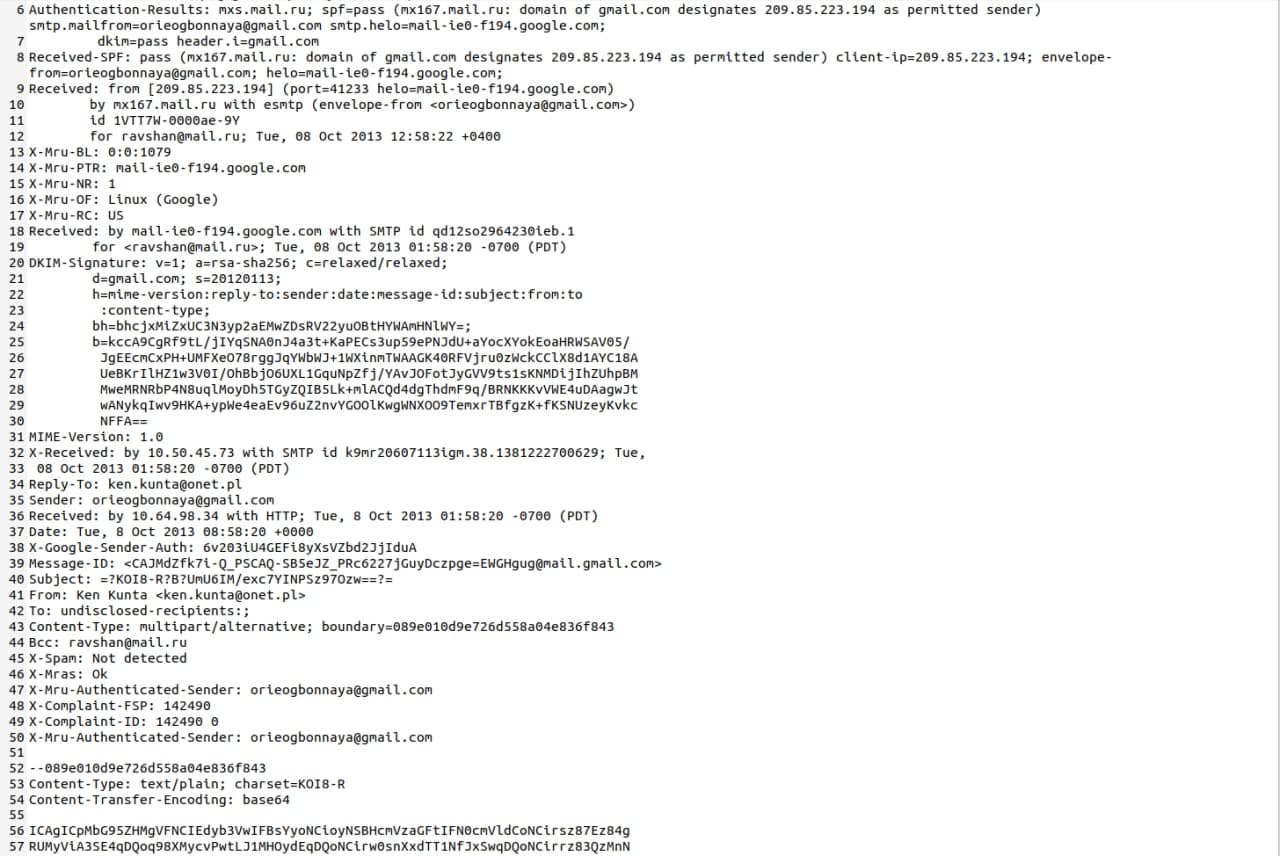
\includegraphics[width=.9\textwidth]{eml_raw.jpg}
\end{center}

\end{frame}

%%%%%%%%%%%%%%%%%%%%%%%%%%%%%%%%%%%%%%
\begin{frame}
\frametitle{Предобработка}

\textbf{Текстовая информация}

Для извлечения информации из документов, имеющих текстовый формат, таких как docx, html, calendar и.т.д. реализованы собственные специализированные парсеры написанные на $C$++

\textbf{Графическая информация}

Поскольку изображения и pdf не являются текстовыми форматами, то
для автоматического извлечения текста разработано два алгоритма машинного обучения на языке Python
\begin{itemize}
\item Модель сегментации и зондирования
\item Модель извлечения текста
\end{itemize}

\end{frame}

%%%%%%%%%%%%%%%%%%%%%%%%%%%%%%%%%%%%%%
\begin{frame}
\frametitle{Предобработка}

После извлечения информации из всех вложений письма текст проходит через следующие этапы:
\begin{itemize}
\item Конкатенация всех частей с заданными разделителями.
\item Декодирование в заданную кодировку (UTF8, CP1251) и приведение к одному регистру.
\item Удаление лишних пробелов, отступов и стоп--слов.
\item Нормализация
\begin{enumerate}
\item Стемминг
\item Лемматизация
\end{enumerate}
\end{itemize}

\end{frame}

%%%%%%%%%%%%%%%%%%%%%%%%%%%%%%%%%%%%%%
\begin{frame}
\frametitle{Векторизация}

\begin{center}
Векторизация
\end{center}

\end{frame}

%%%%%%%%%%%%%%%%%%%%%%%%%%%%%%%%%%%%%%
\begin{frame}
\frametitle{Мешок слов (bow)}

Каждому слову или словосочетанию (терму) ставится в соответствие некоторое число. В этом случае текст определяется вектором $\vec{w} = (w_1, ..., w_N)^T$,
где $N$ --- размерность из конечного словаря $X^l$ состоящего из уникальных термов обучающей выборки. \\
$w_i$ определяется как Булевский вес:
$$
w_i = \begin{cases}
1, & \mbox{если элемент присутствует в письме}, \\
0, & \mbox{если элемент не присутствует в письме}.
\end{cases}
$$

\begin{center}
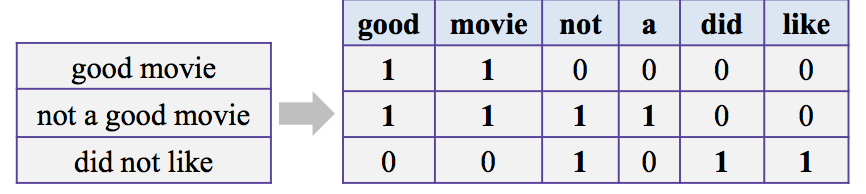
\includegraphics[width=0.6\textwidth]{bow.png}
\end{center}

Основной проблемой bow--векторизации является потеря контекстной связи между словами.

\end{frame}

%%%%%%%%%%%%%%%%%%%%%%%%%%%%%%%%%%%%%%
\begin{frame}
\frametitle{word2vec}

\end{frame}

%%%%%%%%%%%%%%%%%%%%%%%%%%%%%%%%%%%%%%
\begin{frame}
\frametitle{Классификация}

\begin{center}
Классификация
\end{center}

\end{frame}

%%%%%%%%%%%%%%%%%%%%%%%%%%%%%%%%%%%%%%
\begin{frame}
\frametitle{Запуск на пользователях}

\begin{center}
Запуск на пользователях
\end{center}

\end{frame}

%%%%%%%%%%%%%%%%%%%%%%%%%%%%%%%%%%%%%%
\begin{frame}
\frametitle{Заключение}

\begin{center}
Выводы
\end{center}

\end{frame}

%%%%%%%%%%%%%%%%%%%%%%%%%%%%%%%%%%%%%%
\begin{frame}
\frametitle{Заключение}

Публикации
\begin{center}

\end{center}

\end{frame}

%%%%%%%%%%%%%%%%%%%%%%%%%%%%%%%%%%%%%%
\begin{frame}

\frametitle{Заключение}

\begin{center}
СПАСИБО ЗА ВНИМАНИЕ!
\end{center}

\end{frame}

\end{document}
